% !TEX root = ../main.tex
\chapter{Testing}
\label{Testing}

The final product of this project should be a realistic simulation of a Decentralised Community Energy System. To produce the simulation, each of the following features will be tested to ensure they work individually and together:

\begin{itemize}
\item Agents are able to submit their requests to the Virtual Agent they are connected to.
\item Virtual Agents are able to submit their requests to the Supervisor.
\item Virtual Agents and their Agents are allocated Generation dispatch and an amount of electricity to use 
\end{itemize}

Due to time constraints, unit testing was not implemented. A series of tests was done manually by exporting the data using Excel to prove that the simulator was working as intended. The testing has been outlined in the sections below. Each of the tests below has been conducted for the following simulation cases:

\begin{itemize}
	\item 1 Supervisor, 1 Virtual Agent and 1 Agent
	\item 1 Supervisor, 2 Virtual Agent and 2 Agents (Each Virtual Agent connected to 1 Agent)
	\item 1 Supervisor, 2 Virtual Agents and 4 Agents (Each Virtual Agent connected to 2 Agents)
	\item 1 Supervisor, 5 Virtual Agents and 25 Agents (Each Virtual Agent connected to 5 Agents)
\end{itemize}

\section*{Testing Request Submission} % (fold)
To test that Agents are able to submit their Demand and Generation requests, the individual Demand and Generation request of each Agent was recorded in a CSV file. The allocations in the CSV file was summed and compared to that of the computed Global Demand and Generation request.

An example can be seen in figure \ref{fig:test1} of testing the contribution of 25 Agents during hour 23 of a simulation

\clearpage

\begin{figure}[h!]
	\centering
	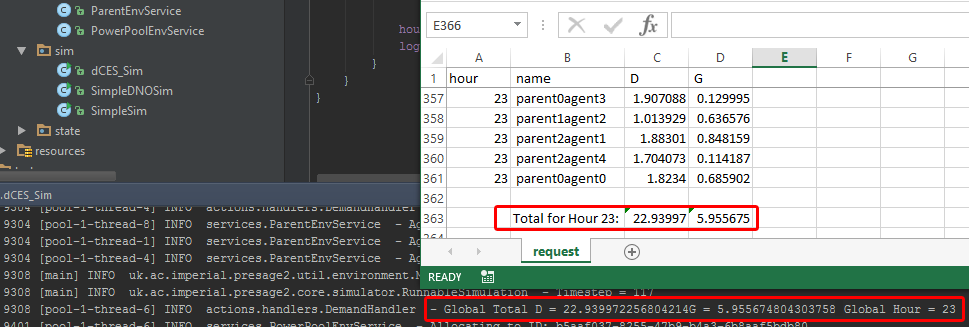
\includegraphics[scale=0.4]{Images/test-contribution.png}
	\caption{Testing the contribution at hour 23 of the simulation for 25 Agents}
	\label{fig:test1}
\end{figure}



\section*{Testing Allocation Algorithm}
When the global aggregated Generation requests exceed the global aggregated Demand requests, all Agents are expected to receive their requests. Globally, Generation is curtailed to not exceed total Demand Request. Generation is curtailed proportionally for everyone. In this case, we should expect all Agents to be allocated less Generation than they have requested, and all Agents to be allocated their Demand requests. An example of this test being passed can be seen in figure \ref{fig:test2}. \\

\begin{figure}[h!]
	\centering
	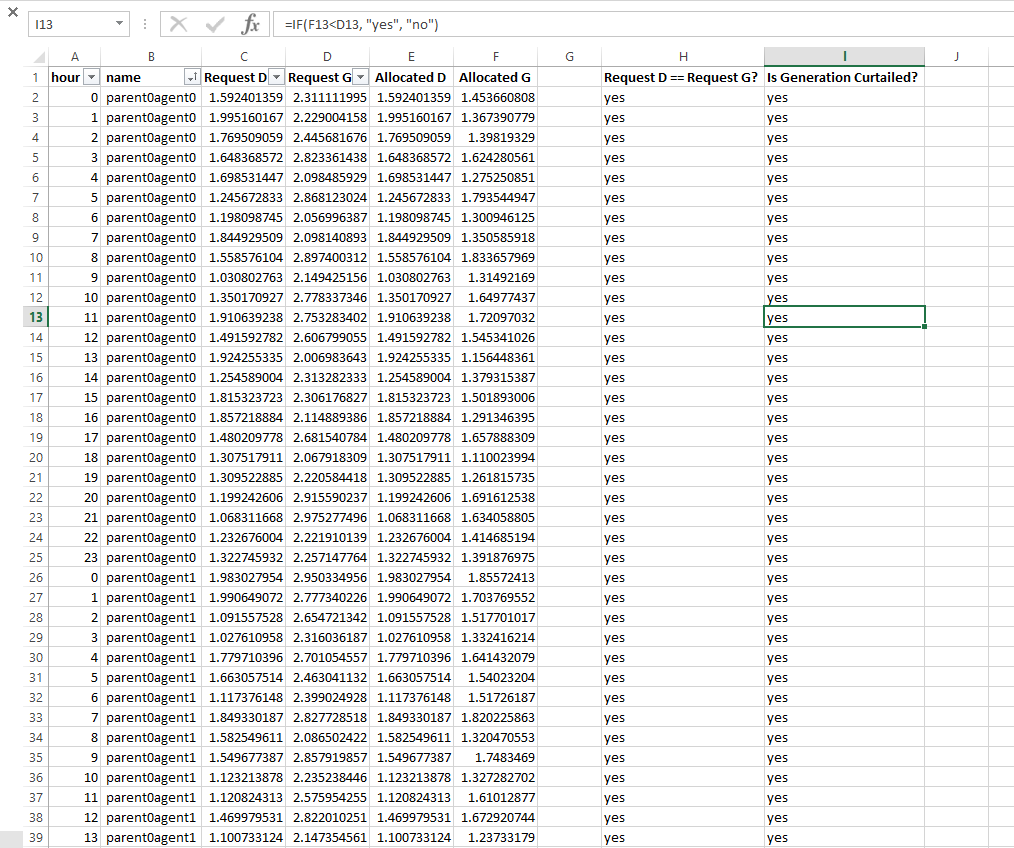
\includegraphics[scale=0.4]{Images/test-allocation1.png}
	\caption{Testing the allocation of 25 Agents when total Generation Request Exceeds total Demand Request}
	\label{fig:test2}
\end{figure}

When the global aggregated Demand request exceed the global Demand request, the fair allocation method will need to be used. To ensure this is working as intended, we need to ensure the following tests are passed:

\begin{enumerate}
	\item Total allocated Demand is equal to total allocated Generation
	\item Total allocated Generation is equal to the total Generation request
	\item Demand allocation proportion is correct
	\item Borda ranking is correct for each of the canons
	\item Borda voting by the Agents are correct
	\item Borda voting is taken into consideration in the next round
\end{enumerate}

\subsection*{Tests 1 and 2}
To check that total allocated Demand is equal to total Generation dispatch, and the total Generation dispatch is equal to the total Generation request, the total Generation Request, Generation Dispatch and Demand Allocation were summed up for each hour of the simulation.  Figure \ref{fig:test3} shows the data for one of such tests. The summation at the bottom shows that the total allocated Demand (Allocated D) and Generation Dispatch (Allocated G) is equal to the total requested Generation (Request G).

\begin{figure}[h!]
	\centering
	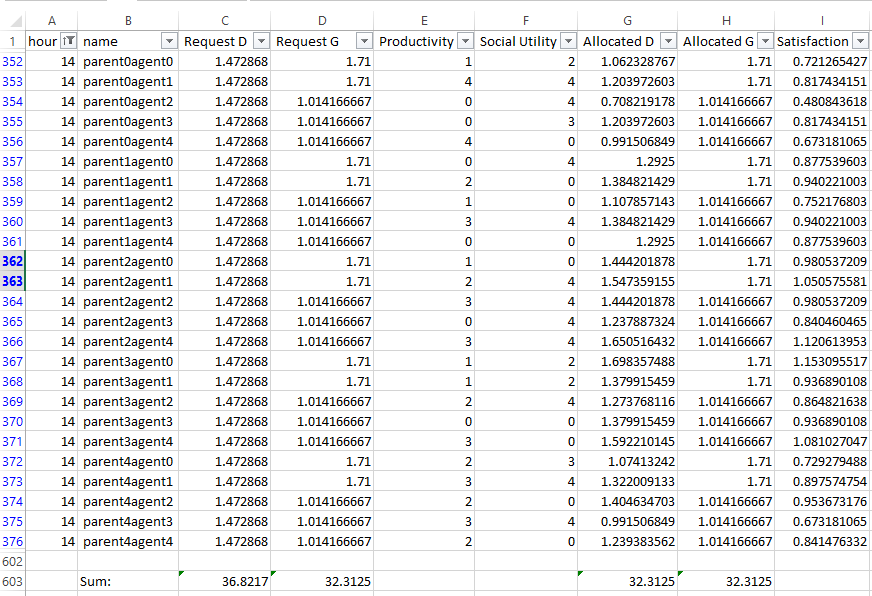
\includegraphics[scale=0.4]{Images/test-allocation2.png}
	\caption{Checking that Allocated Demand is less than total Allocated Generation}
	\label{fig:test3}
\end{figure}

\subsection*{Test 3}
To test that the allocation proportion is correct, Borda ranking and point allocation for each Agent under each of the canons need to be checked to be correct. Figure \ref{fig:test4} shows the previous requests and allocations made by Agents under Virtual Agent \textit{Parent0}. Figure 

\begin{figure}[h!]
 	\centering
 	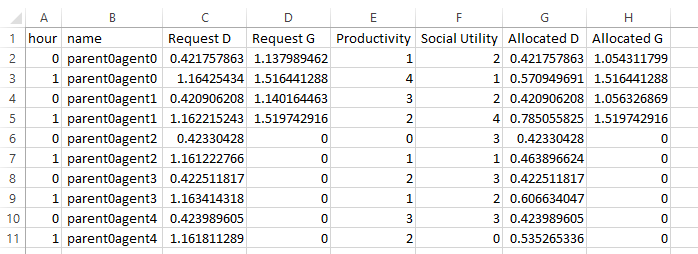
\includegraphics[scale=0.4]{Images/test-allocation3(PrevData).png}
 	\caption{Parent0 Agent requests and allocations}
 	\label{fig:test4}
 \end{figure} 

 \begin{figure}[h!]
 	\centering
 	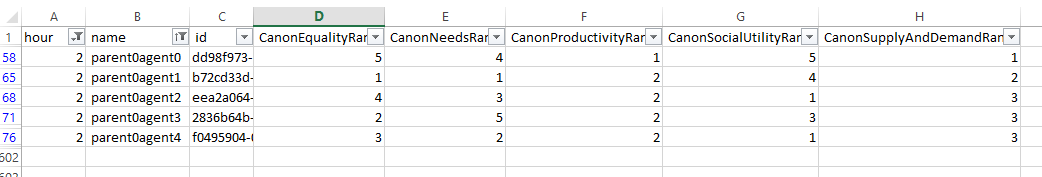
\includegraphics[scale=0.4]{Images/test-allocation3(Ranking).png}
 	\caption{Parent0 Agent ranking}
 	\label{fig:figure1}
 \end{figure}

% section section_name (end)
%If data is available for the potential customers in Rugaragara, the simulation could be used in %conjunction with the feasibility study